\section{実験方法}
\label{sec:methods}
本実験では,ポリアクリルアミド(PAA)溶液(三菱ケミカル,AP805C)を擬塑性流体として用いた.初めに,試験溶液であるPAA溶液を作製し,非ニュートン流体における指標の一つとなる粘度の計測を行うことで粘度特性を計測した.また,応力と貯蔵弾性率,損失弾性率の計測を行うことで,応力に対する弾性特性を計測した.続いて,超音波振動子によって圧力場が適切に生成されているか確認した.そして,擬塑性流体中を落下する球に対する超音波照射による影響を調べるため,球落下実験を行った.

\subsection{実験系および座標系}
\label{sec:exp-system}
本研究における実験系および座標系をFig.\ref{fig:system}に示す.本研究で扱う系は,水槽中において,超音波照射された擬塑性流体中を球が落下する系である.水槽液面を原点とし,球の落下方向をy軸正の方向とする.

\begin{figure}[H]
    \centering
    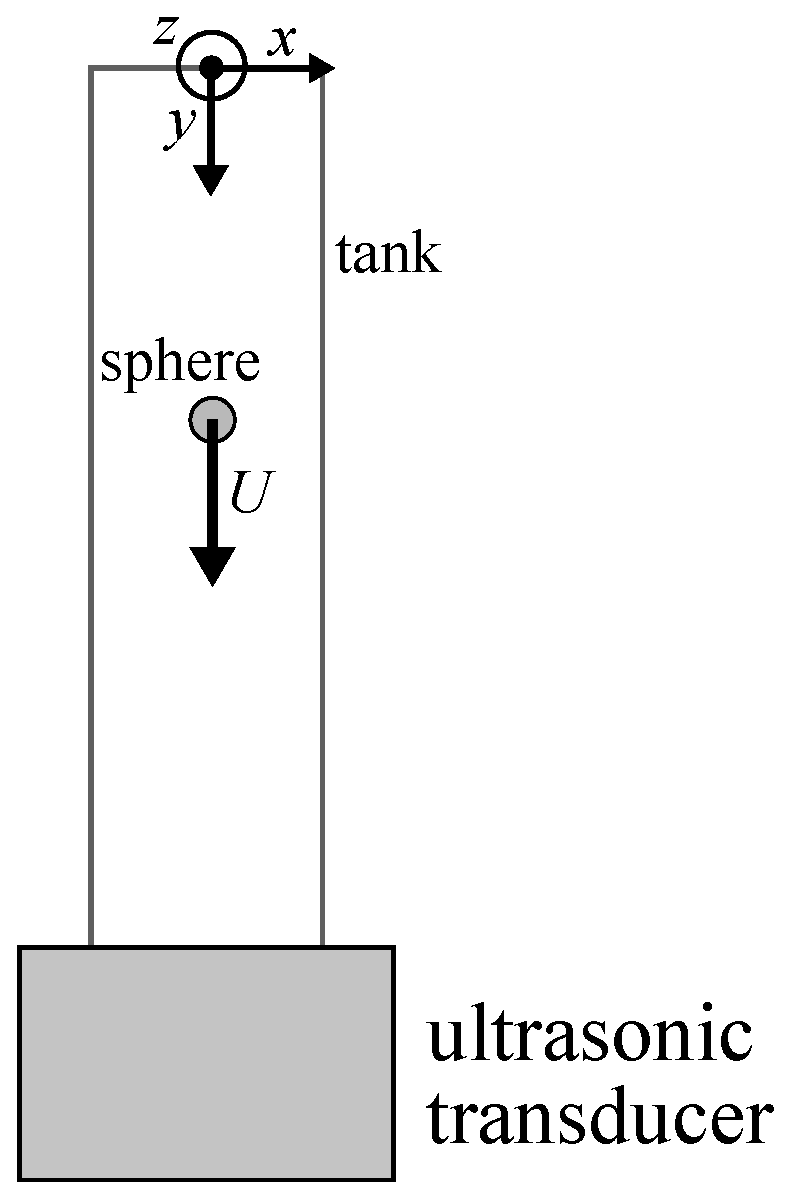
\includegraphics[width=0.32\textwidth]{./2-Methods/device-coordinate.eps}
    \caption{Experimental system and coordinate system.}
    \label{fig:system}
\end{figure}

\subsection{溶液作製}
PAA粉末と水道水を混合することで,全7種類の濃度(0.05,0.2,0.5,0.7,1.0,1.3,1.5wt.\%)のPAA溶液を作製した.以下にその作製方法を示す.

はじめに,1Lポリビーカー空容器質量をデジタルスケールを用いて計測を行った.そこに約1Lの水道水を入れ再度デジタルスケールで質量の計測を,水道水の質量の算出した.この結果より,作製する濃度に必要なPAA粉末の質量を算出し,デジタルスケールで計量を行った.このPAA粉末を水道水の攪拌を行いながら少量ずつ混合させた.これは溶液全体で均一性を持たせるためである.そして,マグネットスチーラー,プラスチック製攪拌棒を用いて溶液の攪拌を行った.これらを2回行うことで1度に約2LのPAA溶液の作製を行った.作製約1週後,溶液に気泡が見られなくなった後,ペットボトル容器に移し密封保管を行った.これは,水分の蒸発を防ぎ,濃度が大きく変化することを防ぐためである.

\subsection{粘度計測}
粘度計測における計測機器の模式図をFig.\ref{fig:viscosity}に示す.ステージと回転する円錐回転子の間に存在する試料によって付加されるトルクを計測することで粘度の計測を行う.粘度のせん断速度依存性を確認することで生成した溶液の性質の確認を行った.なお、計測範囲の都合上、水道水では1°34′×R24のコーンロータを,PAA溶液では0.8°×R12のコーンロータをそれぞれ用いた.コーンロータを用いることで,試料全域に同じひずみ速度を与えた.

\begin{table}[h]
    \centering
    \caption{Specifications of viscometer(東機産業,TVE-25L)}
    \label{table:viscometer}
    \begin{tabular}{c|c}\hline
        測定方式    & 円錐平板方式                    \\ \hline
        回転速度    & 0,0.1~100.0rpm;0.1rpmステップ \\ \hline
        精度/再現性 & \begin{tabular}{c}
                          フルスケールの±1.0\%以内/ \\
                          フルスケールの±0.2\%以内
                      \end{tabular}       \\ \hline
    \end{tabular}
\end{table}
\begin{center}
    \begin{figure}[H]
        \centering
        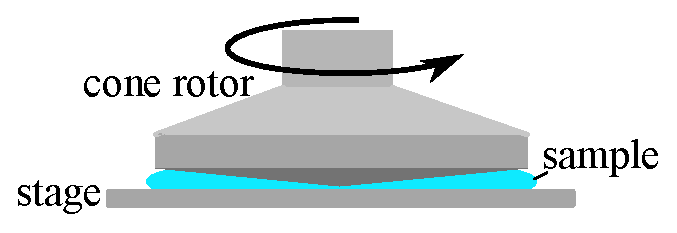
\includegraphics[width=0.5\textwidth]{2-Methods/Viscosity-Measurement.eps}
        \caption{Viscosity measurement method.}
        \label{fig:viscosity}
    \end{figure}
\end{center}

\subsection{弾性率計測}

作製したPAA溶液の応力に対する弾性特性を調べるため,貯蔵弾性率$G'$と損失弾性率$G''$の応力依存性を計測した.以下に,その計測理論と計測手法を示す.

\subsubsection{弾性率 計測理論}
周期的なひずみを試験溶液に印可し,そのときの応力を計測することで貯蔵弾性率$G'$と損失弾性率$G''$の計測を行う.試験溶液にひずみが,
\begin{eqnarray}
    \gamma=\gamma_1e^{i\omega{}t} ,
\end{eqnarray}
で与えられたとする.粘弾性体では,ひずみは応力に対して位相が遅れるので,応力はひずみより位相が進む.印可されたひずみと応力の関係をFig.\ref{fig:elastcity}に示す.位相差を$\eta$とすると,
\begin{eqnarray}
    \tau=\tau_1e^{i\left(\omega{}t+\eta\right)} ,
    \label{eq:tau_gamma}
\end{eqnarray}
となる.ここで,
\begin{eqnarray}
    |G| &=& \frac{\tau_1}{\gamma_1} ,
\end{eqnarray}
とおくと,式(\ref{eq:tau_gamma})は,
\begin{eqnarray}
    \tau=\gamma_1|G|e^{\left(\omega{}t+\eta\right)}=|G|\gamma{}e^{i\eta} ,
    \label{eq:tau_G}
\end{eqnarray}
と表される.ここで,
\begin{eqnarray}
    G^* &=& \frac{\tau}{\gamma}\\
    G' &=& |G|\cos\eta ,\label{eq:G_prime}\\
    G'' &=& |G|\sin\eta ,\label{eq:G_doubleprime}
\end{eqnarray}
とおくと,式(\ref{eq:tau_G})は,
\begin{eqnarray}
    G^* = |G|e^{i\eta} ,
    \label{eq:G_star}
\end{eqnarray}
となる.ここで,式(\ref{eq:G_prime}),(\ref{eq:G_doubleprime})より,
\begin{eqnarray}
    G^* = G'+iG'' ,
\end{eqnarray}
となる.ここで,$G^*$は複素弾性率,$G'$は貯蔵弾性率,$G''$は損失弾性率と呼ばれる\cite{生物レオロジー}\cite{化学者のためのレオロジー}.貯蔵弾性率と損失弾性率に関して,位相差$\eta$を用いて,
\begin{alignat}{3}
    G' & = 0 ,           & \quad G'' & = |G| ,         & \quad & \left(\text{at } \eta=0\right)               \label{eq:G_case1} \\
    G' & = |G|\cos\eta , & G''       & = |G|\sin\eta , &       & \left(\text{at } 0<\eta<\frac{\pi}{2}\right) \label{eq:G_case2} \\
    G' & = |G| ,         & G''       & = 0 ,           &       & \left(\text{at } \eta=\frac{\pi}{2}\right)   \label{eq:G_case3}
\end{alignat}
とそれぞれの条件で場合分けできる.式(\ref{eq:G_case1})の場合は,応力とひずみの位相差が存在せず,粘性による影響がなく,弾性による影響のみが存在する.式(\ref{eq:G_case3})の場合は,応力とひずみの位相差が$\pi/2$で直交し,弾性による影響がなく,粘性による影響のみが存在する.式(\ref{eq:G_case2})の場合は,応力とひずみの位相差が$\pi/2$より小さいが存在し,弾性,粘性それぞれの影響を受けることを示している.以上より,損失弾性率$G'$は粘性影響を,貯蔵弾性率$G''$は弾性影響を表すことが分かる.式(\ref{eq:G_prime}),(\ref{eq:G_doubleprime})より,損失弾性率と貯蔵弾性率の比を
\begin{eqnarray}
    \frac{G''}{G'} &=& \tan\eta ,
    \label{eq:loss_factor}
\end{eqnarray}
と定義できる.ここで,$\tan\eta$は損失正接と呼ばれる\cite{生物レオロジー}\cite{化学者のためのレオロジー}.この損失正接に関して,
\begin{alignat}{2}
    \tan\eta & < 1, & \quad \left(\text{at } 0<\eta<\frac{\pi}{4}\right)     \label{eq:tan_eta_case1}         \\
    \tan\eta & > 1, & \quad \left(\text{at } \frac{\pi}{4}<\eta<\frac{\pi}{2}\right) \label{eq:tan_eta_case2}
\end{alignat}
と,場合分けできる.式(\ref{eq:tan_eta_case1})の場合は,貯蔵弾性率よりも損失弾性率の方が大きく,粘性による影響を強く受ける.一方で,式(\ref{eq:tan_eta_case2})の場合は,損失弾性率より貯蔵弾性率の方が大きく,弾性による影響を強く受ける.本研究において,損失正接を用いた場合分けによって粘性影響,弾性影響を考えた.

\begin{figure}[ht]
    \centering
    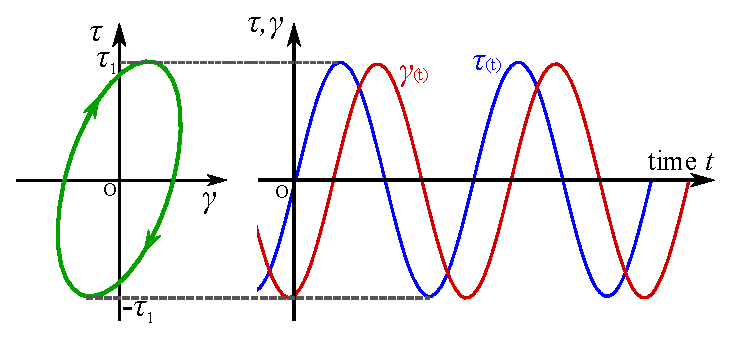
\includegraphics[width=0.75\textwidth]{2-Methods/elasticity.eps}
    \caption{Relationship between shear rate and stress in viscoelastic materials.}
    \label{fig:elastic}
\end{figure}

\newpage

\subsubsection{弾性率 計測手法}

弾性率計測の概略図をFig.\ref{fig:elastic-measure}に示す.計測には,回転式レオメータ(Thermo Fisher Scientific,HAAKE MARS$\rm I\hspace{-.15em}I\hspace{-.15em}I$)を用いた.回転子の振動回転周期を一定にし,振幅を変化させることで溶液に印可する応力を変化させた.回転子には1°×R30のコーンロータを用いた.計測条件をTable\ref{table:elastic}に示す.

\begin{table}[ht]
    \centering
    \caption{Elastic modulus measurement conditions.}
    \label{table:elastic}
    \begin{tabular}{c|c}\hline
        計測範囲     & $10^{-3} \sim 10^3$[Pa] \\ \hline
        計測分割数   & 70                      \\ \hline
        計測分割形式 & 対数                    \\ \hline
        計測温度     & 20[$^\circ$C](固定)   \\ \hline
        回転子周期   & 1[Hz](固定))         \\ \hline
    \end{tabular}
\end{table}

\begin{figure}[ht]
    \centering
    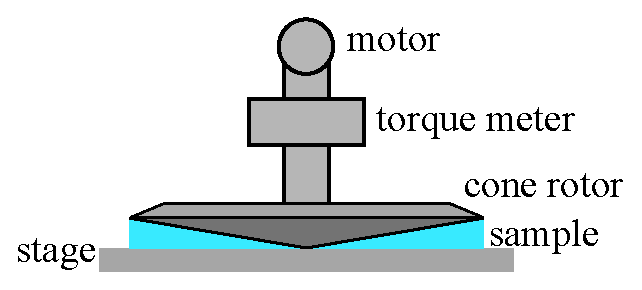
\includegraphics[width=0.7\textwidth]{2-Methods/rheometer.eps}
    \caption{Elastic modulus measurement conditions.}
    \label{fig:elastic-measure}
\end{figure}

\newpage

\subsection{圧力場計測}

圧力場計測の概略図を\ref{fig:microphone}に示す.圧力測定にはハイドロフォン(Br\"{u}el \& Kj\ae r,Hydrophone Type8103)を用いた.ハイドロフォンの出力電圧をコンディショニングアンプ(Br\"{u}el \& Kj\ae r,NEXUS Change Amplifier Type 2692-A-0S1)を用いて増幅し,オシロスコープを用いて電圧を記録した.コンディショニングアンプの設定を元に記録した電圧を圧力場へ変換した.計測は5mm間隔で行った.この測定間隔は音速$c\approx \SI{1500}{m/s}$,周波数$f=\SI{27.4}{kHz}$としたときの波長$\lambda=c/f\approx \SI{54.7}{mm}$よりも十分に小さい.

\begin{table}[ht]
    \centering
    \caption{Specifications of microphone (Br\"{u}el \& Kj\ae r,Hydrophone Type8103)}
    \label{table:microphone}
    \begin{tabular}{c|c}\hline
        公称電圧感度 & 29$\mu$V/Pa   \\ \hline
        計測範囲     & 0.1kHz-180kHz \\ \hline
    \end{tabular}
\end{table}

\begin{table}[ht]
    \centering
    \caption{Specifications of conditioning amplifier(Br\"{u}el \& Kj\ae r,NEXUS Change Amplifier Type 2692-A-0S1)}
    \label{table:conditioning amplifier}
    \begin{tabular}{c|c}\hline
        マイクロフォン入力 &                                   \\ \hline
        入力インピーダンス & 10M$\Omega$\textbar \textbar300pF \\ \hline
        最大入力           & 31.6V                             \\ \hline
        周波数範囲(-1dB) & 0.1kHz-100kHz(ゲイン$\leq$60dB)   \\ \hline
    \end{tabular}
\end{table}

\begin{figure}[H]
    \centering
    \label{fig:microphone}
    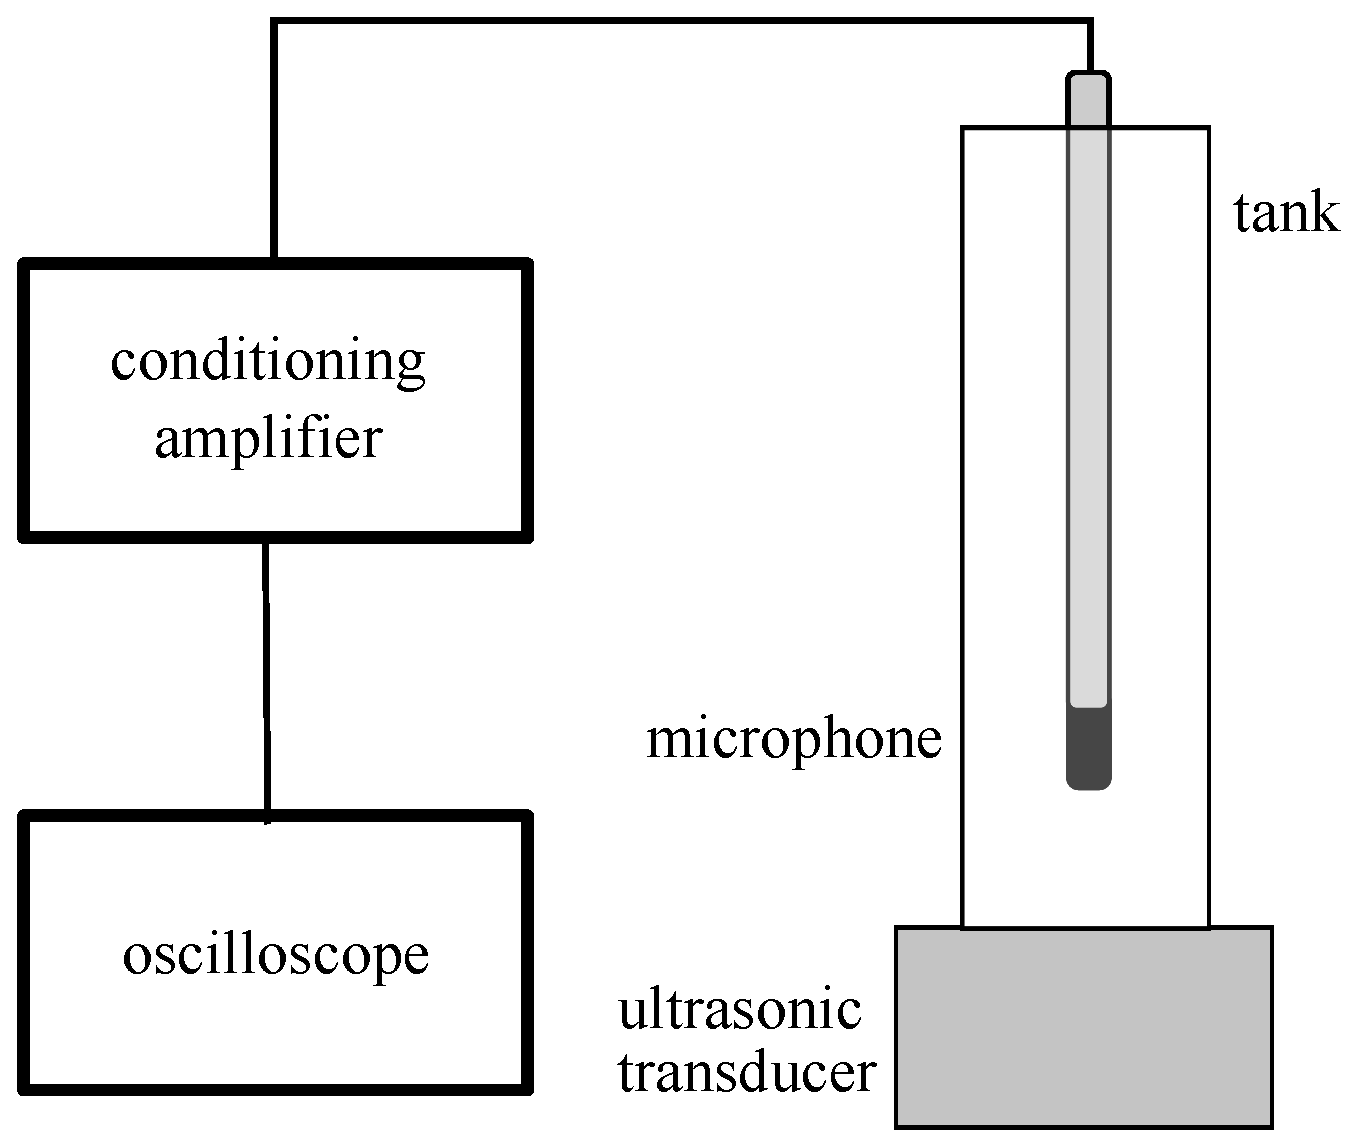
\includegraphics[width=0.7\textwidth]{2-Methods/microphone.eps}
    \caption{Schematic outline for pressure measurement.}
\end{figure}

\subsection{球落下実験}

使用した実験装置の概略図をFig.\ref{fig:device}に示す.外寸にて高さ400mm,幅58mm,奥行き58mm,厚さ3mmの矩形アクリル水槽を用いた.この水槽に試験溶液を満たした.その上に,真空ポンプと接続した真空パッドを設置し,直径$D$の球の保持をした.三方弁を用いて真空パッドを大気圧にすることで落下球の把持を解除し,球を落下させた.密度,濃度変化の場合における落下球,溶液の条件をTable.\ref{table:exp-conditions}に示す.また,落下球の球径を変化させた場合の球径,溶液の濃度の条件をTable.\ref{table:exp-conditions-dia}に示す.落下させた球が鋼球の場合は,ネオジム磁石を用いて試行ごとに回収を行った.一方で,他の種類の球は回収せずに落下実験を継続した.この際,落下球の体積によって液面が上昇するので液面の高さが一定になるよう,シリンジを用いて溶液を回収した.

落下球が試験液体中を落下する様子をハイスピードカメラ(BASLER, acA1920-150um)で撮影し,記録用コンピュータに連続画像(bmp形式)として保存した.解像度は0.22mm/pixelであり,最小の球(直径5mm)でも直径22.7pixelの円として撮影できる.ハイスピードカメラにはレンズ(BASLER, TS5014-MP)をつけ,絞り,焦点の調整を行い,明瞭に落下球を撮影できるようにした.実験装置後方にスクリーン,赤外線ライトを設置し,装置を後方より照射することにより,落下の様子をより分かりやすくした.さらに,超音波振動による影響を調査するためにアクリル水槽の下に超音波振動子を設置した.

\begin{figure}[h]
    \centering
    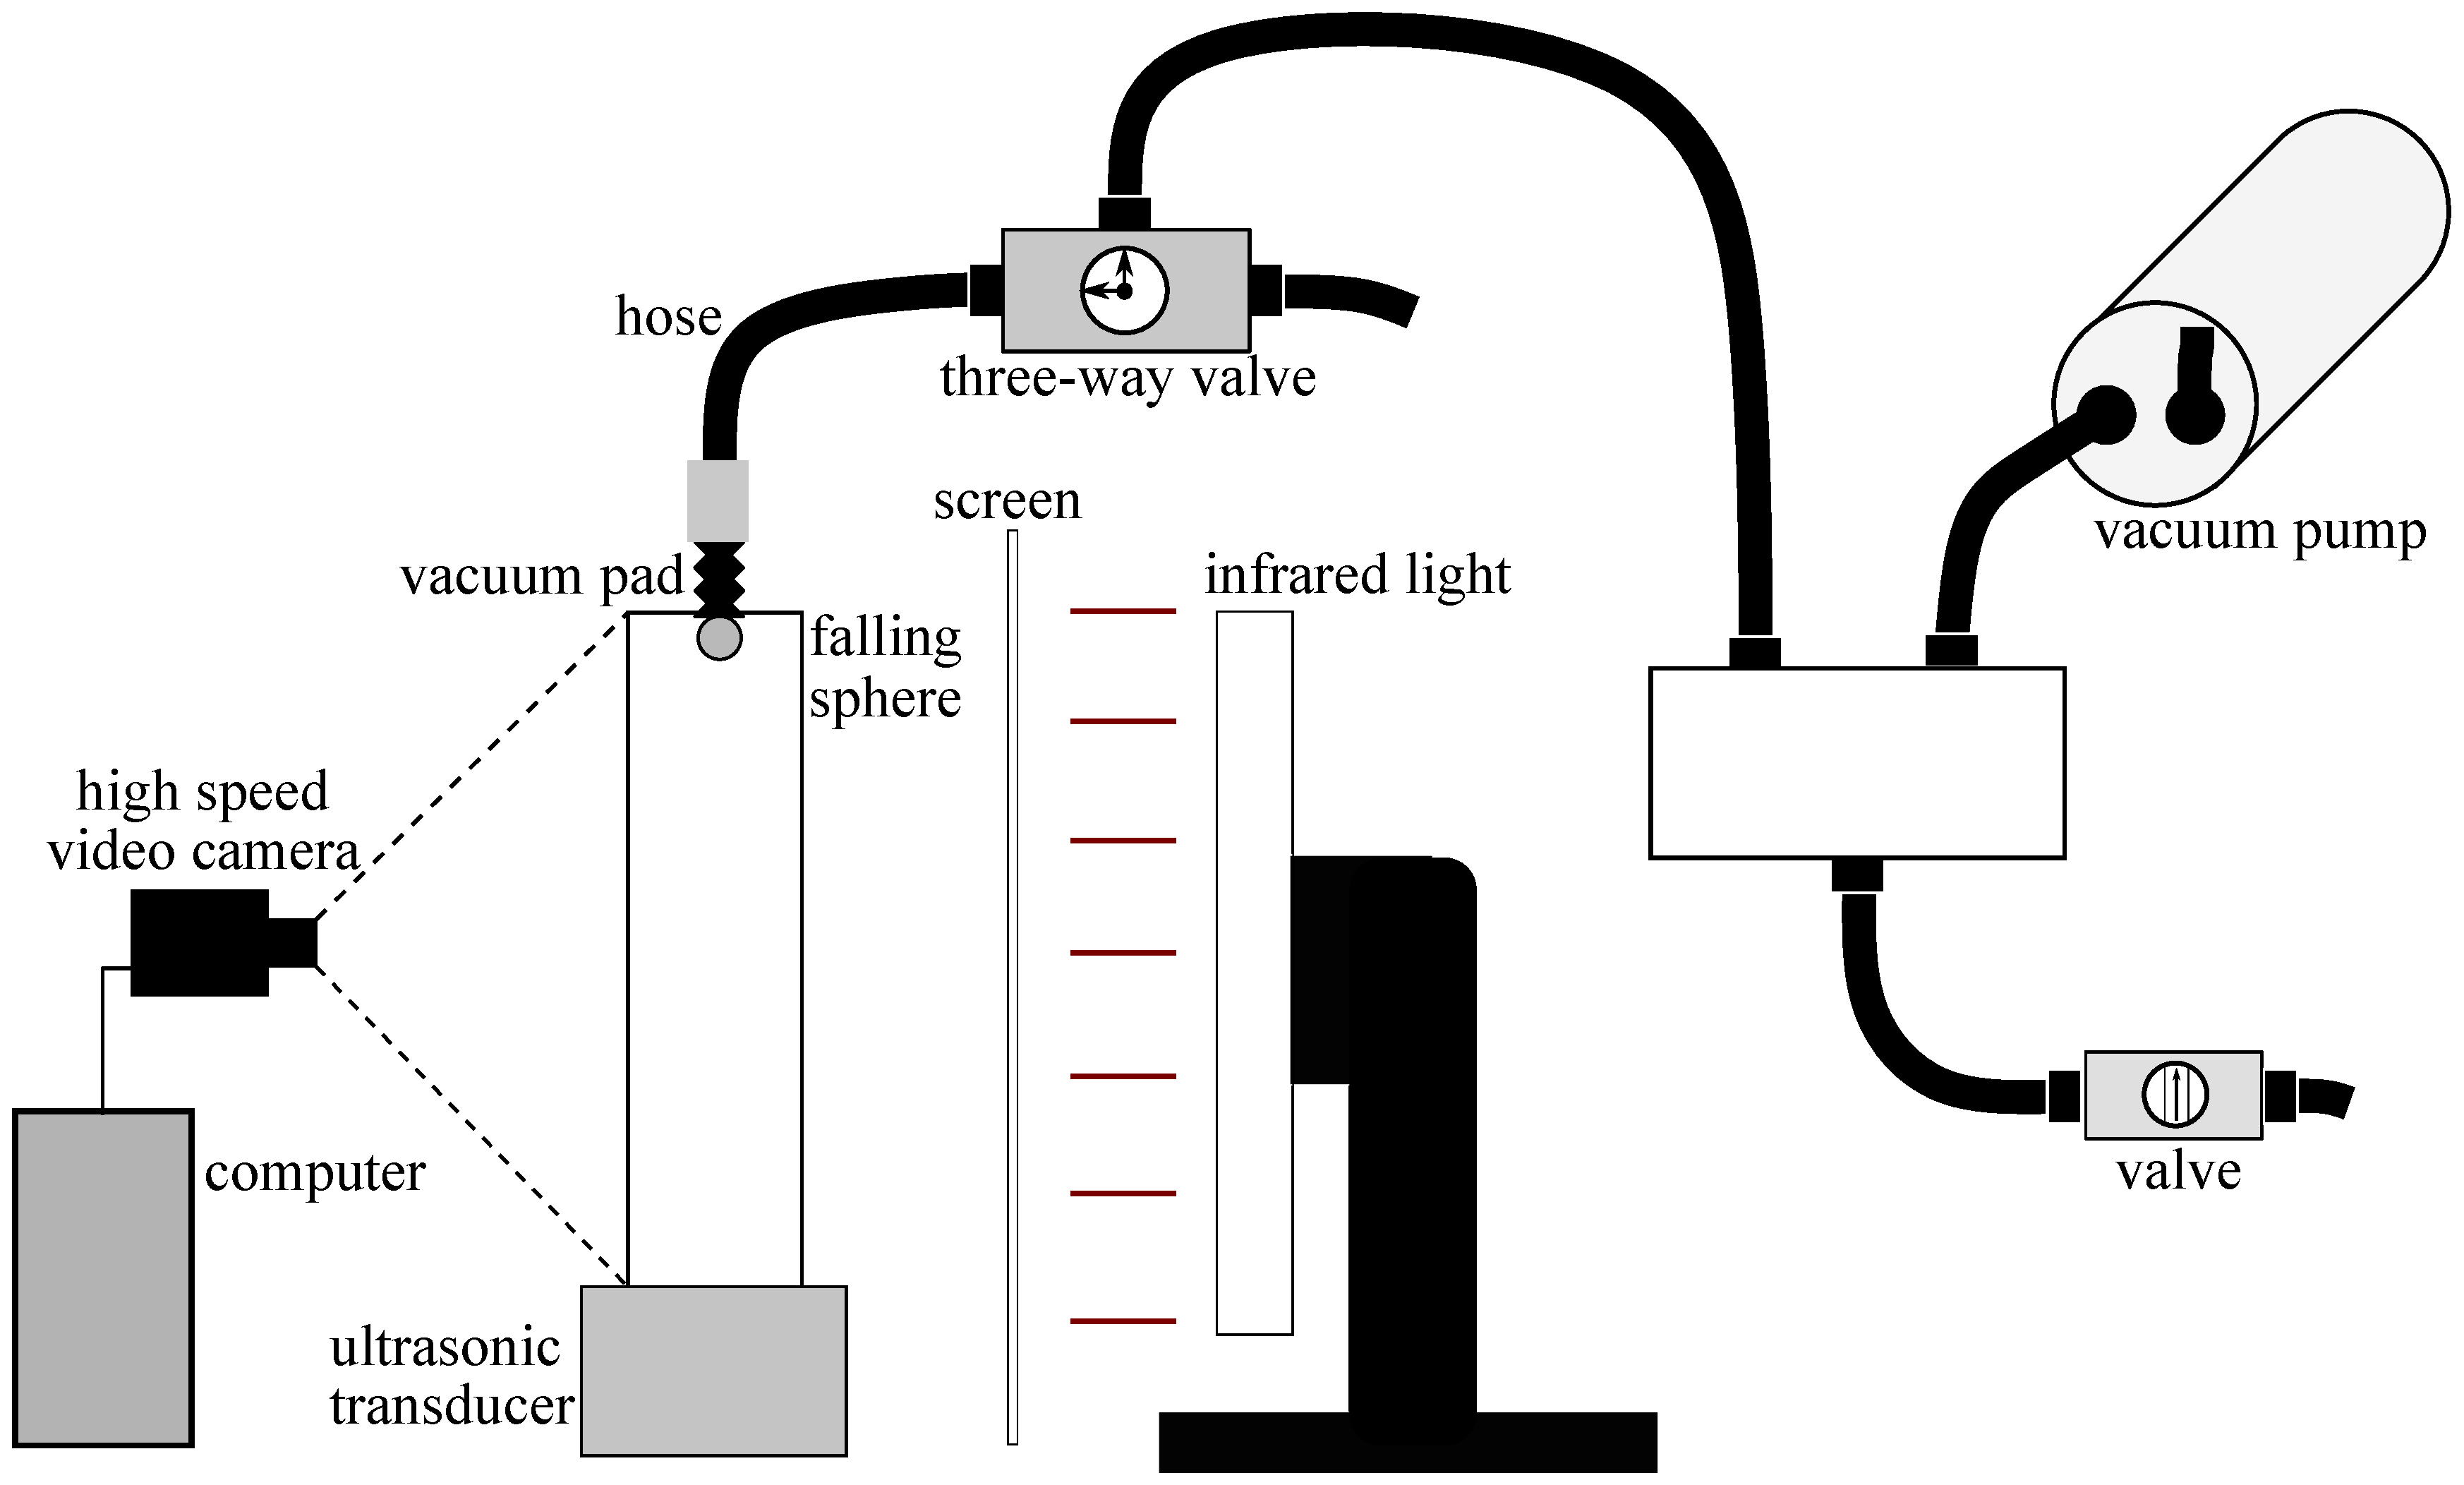
\includegraphics[width=0.9\textwidth]{2-Methods/device-vacuum.eps}
    \caption{Schematic view of the experimental apparatus.}
    \label{fig:device}
\end{figure}

\begin{table}[h]
    \centering
    \caption{Specifications of high-speed camera (BASLER, acA1920-150um)}
    \label{table:camera}
    \begin{tabular}{c|c}\hline
        センサ種別      & CMOS                      \\ \hline
        水平/垂直解像度 & 200pixel$\times$1984pixel \\ \hline
        解像度          & 0.5MP                     \\ \hline
        フレームレート  & 100fps                    \\ \hline
    \end{tabular}
\end{table}

\begin{table}[ht]
    \centering
    \caption{Specifications of lens (BASLER, TS5014-MP)}
    \label{table:lens}
    \begin{tabular}{c|c}\hline
        焦点距離[mm]     & 50.0     \\ \hline
        F値              & 1.4-16.0 \\ \hline
        最短撮影距離[mm] & 500      \\ \hline
    \end{tabular}
\end{table}

\begin{table}[H]
    \centering
    \caption{Experimental conditions of falling sphere and solution concentration.}
    \label{table:exp-conditions}
    \begin{tabular}{c|c|c|c|c|c|c}\hline
        球材質                & nylon   & アルミニウム & アルミナ & 鋼      & ステンレス & 真鍮    \\ \hline
        密度 $\rho$[kg/m$^3$] & 1130    & 2700         & 3800     & 7900    & 7900       & 8700    \\ \hline
        直径 $D$[mm]          & 9.5     & 10           & 10       & 10      & 9.525      & 9.52    \\ \hline \hline
        PAA 0.05wt.\%         & $\circ$ &              &          &         &            &         \\ \hline
        PAA 0.2wt.\%          &         & $\circ$      & $\circ$  &         & $\circ$    & $\circ$ \\ \hline
        PAA 0.5wt.\%          &         & $\circ$      & $\circ$  &         & $\circ$    & $\circ$ \\ \hline
        PAA 0.7wt.\%          &         & $\circ$      & $\circ$  &         & $\circ$    & $\circ$ \\ \hline
        PAA 1.0wt.\%          &         & $\circ$      & $\circ$  & $\circ$ &            & $\circ$ \\ \hline
        PAA 1.3wt.\%          &         & $\circ$      & $\circ$  &         & $\circ$    & $\circ$ \\ \hline
        PAA 1.5wt.\%          &         &              & $\circ$  &         & $\circ$    & $\circ$ \\ \hline
    \end{tabular}
\end{table}

\begin{table}[H]
    \centering
    \caption{Experimental conditions on steel sphere with varying sphere diameters.}
    \label{table:exp-conditions-dia}
    \begin{tabular}{c|c|c|c|c|c|c|c|c|c}\hline
        球材質       & \multicolumn{9}{|c}{鋼 $\rho$ =7900kg/m$^3$}                                                                                 \\ \hline
        直径 $D$[mm] & 5                                            & 8       & 10      & 11      & 12      & 13      & 14      & 15      & 20      \\ \hline \hline
        PAA 0.2wt.\% & $\circ$                                      & $\circ$ & $\circ$ &         &         &         &         &         &         \\ \hline
        PAA 0.5wt.\% & $\circ$                                      &         & $\circ$ &         &         &         &         & $\circ$ & $\circ$ \\ \hline
        PAA 1.0wt.\% &                                              & $\circ$ & $\circ$ & $\circ$ & $\circ$ & $\circ$ & $\circ$ & $\circ$ & $\circ$ \\ \hline
        PAA 1.3wt.\% &                                              & $\circ$ & $\circ$ &         &         &         &         & $\circ$ & $\circ$ \\ \hline
    \end{tabular}
\end{table}

超音波振動子の発振には,ファンクションジェネレータ(NF,WF1974),オシロスコープ(IWATSU,DIGITAL OSCILLOSCOPE DS-5614A),パワーアンプ(NF,HSA4101)を用いた.これらの接続をFig.\ref{fig:connect-with-signal}に示す.ファンクションジェネレータによって,周波数,電圧の制御を行い,超音波出力の出力元となる正弦波信号を生成した.続いて,ファンクションジェネレータによって生成された正弦波信号をパワーアンプによって,20倍のゲインをかけ増幅した.これら,オシロスコープによってファンクションジェネレータによって生成された信号,パワーアンプによって増幅された信号の両方をモニタリングし正常に出力されているか確認を行った.また,パワーアンプによって増幅された信号を,ランジュバン型振動子(富士セラミックス,FBL28502HA)上に円形のSUS製プレートを接着したものを振動子とした.超音波振動子の共振周波数は28kHzである.今回の実験において,照射する超音波周波数は27.4kHzに固定した.

\begin{figure}[h]
    \centering
    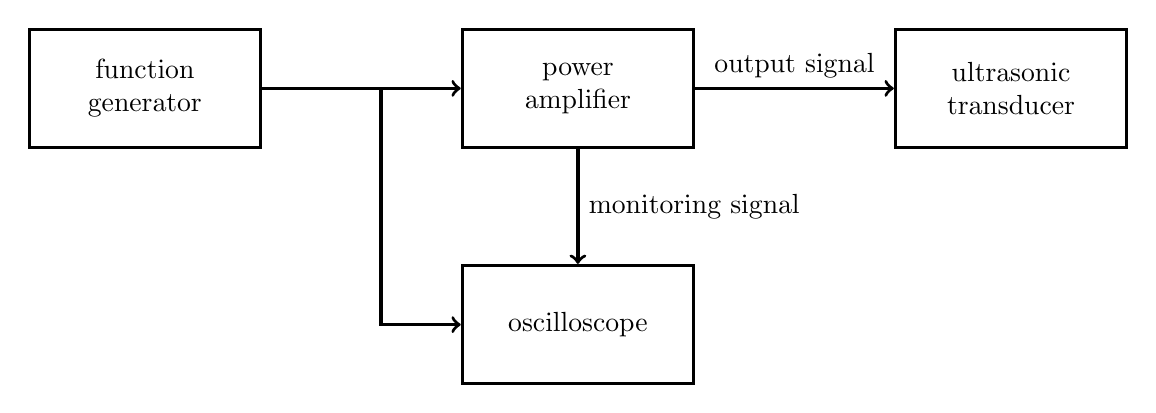
\begin{tikzpicture}[samples=100, very thick]
        \tikzset{rect/.style={rectangle,  draw,  text centered, text width=2.7cm, minimum height=1.5cm}};
        \node[rect](a) at(0,3){function \\ generator};
        \node[rect](b) at(5.5,3){power \\ amplifier};
        \node[rect](c) at(5.5,0){oscilloscope};
        \node[rect](d) at(11,3){ultrasonic \\ transducer};
        \draw[->] (a) -- (b);
        \draw[->] (3,3)--(3,0)--(c);
        \draw[->] (b) -- (c)node[pos=0.5,right]{monitoring signal};
        \draw[->] (b) --(d)node[pos=0.5,above]{output signal};
    \end{tikzpicture}
    \caption{Schematic outline for ultrasonic control system.}
    \label{fig:connect-with-signal}
\end{figure}

\newpage

\subsection{実験手順}

実験手順のフローチャートをFig.\ref{fig:exp-methods}に示す.まず初めに,試験溶液であるPAA溶液の作製を行った.続いて,粘度計測を行い作製したPAA溶液の粘度特性を計測した.その後,圧力場の計測を行い,PAA溶液中に適切に圧力場が形成されているかの確認を行った.そして,球落下実験を行い超音波照射の有無に伴う落下球への影響を調べた.

超音波を照射した落下実験を行う前に,球を数回落下させ,それぞれの試行ごとに速度が一定となることを確認した.そして,超音波照射なしで球落下実験を行い,その後,超音波照射ありにおける球落下実験を行った.超音波照射ありなしを交互に行うことによって,超音波照射による擬塑性流体中を落下する球への影響を確認した.なお,弾性を有する流体は緩和時間を代表時間として,変形した状態から元の状態へ戻ろうとする.各落下実験における流体の状態を同じ状態とするために,等間隔の時間をあけて球の落下を行う必要がある.これは,先行研究\cite{ref:8-5}にて,等間隔の時間で物体を落下させると,落下速度が一定になることが報告されているためである.本実験においては,10分間隔で物体を落下させた.

\begin{figure}[ht]
    \centering
    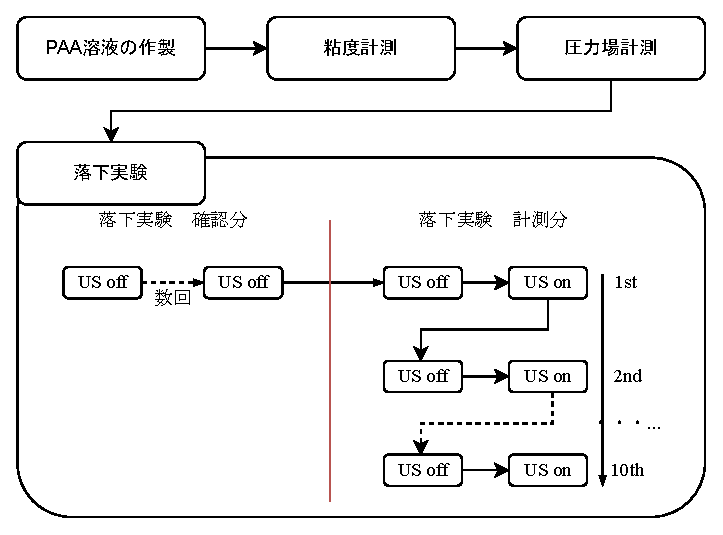
\includegraphics[width=0.7\textwidth]{2-Methods/exp-methods.eps}
    \caption{Flowchart of the experimental procedure.}
    \label{fig:exp-methods}
\end{figure}
